\section{Trivalent Categories}
Trivalent categories, as defined in \cite{Morrison2017Trivalent}, have the nice property that the calculations within are basically calculations in a certain unshaded planar algebra with additional constraints.

We will first write down their category-theoretic definition, but from then on only use string diagrams to apply the methods from the theory of planar algebras. In the vein of the seminal paper we first introduce a few preliminary notions.

The first one is \emph{evaluability}: a monoidal $\mathbb{F}$-linear category is \emph{evaluable} if and only if $\dim\mathrm{Hom}(1,1) = 1$, and that endomorphism space is identified with $\mathbb{F}$ by sending the empty string diagram to $1\in \mathbb{F}$.

Secondly, to rule out a certain degeneracy like before, we call a pivotal category \emph{non-degenerate} iff for every nonzero morphism $f:X\rightarrow Y$ we can find a morphism $f^\prime:Y\rightarrow X$ such that the trace $\mathrm{tr}\left( f^\prime\circ f \right)\in\mathrm{Hom}(1,1)$ is not zero.

For a fixed object $X$ we introduce the notation 
\begin{align*}
\mathcal{C}_n \equiv\mathrm{Hom}\left( 1, X^{\tensor n} \right).
\end{align*}
These vector spaces form an unshaded planar algebra, so far only formally. After the next definition we will understand that $\mathcal{C}_n$ is the span of open planar trivalent graphs with $n$ boundary points, up to isotopy rel boundary, so that only tangles with internal disks of color at most $3$ play any role at all.

\begin{definition}[Trivalent Category]
A triple $\left( \mathcal{C},X,\tau \right)$ forms a \emph{trivalent category} if
\begin{itemize}
\item[•] $\mathcal{C}$ is a strict pivotal $\mathbb{C}$-linear category that is evaluable and non-degenerate
\item[•] $X$ is a self-dual simple object such that 
	\begin{align*}
		\dim\mathcal{C}_1 = 0,\qquad \dim\mathcal{C}_2 = 1,\qquad \dim\mathcal{C}_3 = 1
    \end{align*}
\item[•] $\tau \in \mathcal{C}_3$, called the \emph{trivalent vertex}, is rotationally invariant, that is 
	\begin{align*}
		\begin{tikzpicture}[scale=0.5, baseline]
			\node[draw] (t) at (0,0) {$\tau$};
			\foreach \x in {-0.3,0} \draw ($(t.north) + (\x,0)$) .. controls +(\x,0.5) .. ++(\x,1);
		% 
			\draw ($(t.north) + (0.3,0)$) arc[start angle=180, end angle=0, radius=5mm] --
				++ (0,-1) arc[start angle=0, end angle=-180, radius=1.3cm] -- ++ (0,2);
		\end{tikzpicture}
		\, = \,
			\begin{tikzpicture}[scale=0.5, baseline]
			\node[draw] (t) at (0,0) {$\tau$};
			\foreach \x in {-0.3,0,0.3} \draw ($(t.north) + (\x,0)$) .. controls +(\x,0.5) .. ++(\x,1);
		\end{tikzpicture}\,,
	\end{align*}
	and $\mathcal{C}$ is generated by $\tau$. This means that every morphism is obtained from tensoring and adding identities, (co)evaluations, the self-duality, and trivalent vertices.
\end{itemize}
\end{definition}
Let from now on $\mathcal{C}$ be as in the definition. The object $X$ is actually symmetrically self-dual, meaning that there exists an isomorphism $\phi:X\morphism{\sim} X^*$ with $\phi^* = \phi$. This follows from the non-degeneracy and the dimension of $\mathcal{C}_3$, see Lemma 2.2 in \cite{Morrison2017Trivalent}.

\bigno It is customary to drop the label of the morphism and to simply denote it by a trivalent vertex. Then every string diagram will be an open planar trivalent graph, where strings correspond to simple objects, and two graphs isotopic rel boundary correspond to the same morphism (the self-duality is not drawn). Our category is \emph{defined} to behave nicely, so we can use planar isotopy to deform graphs. For us it is not necessary to reinterpret the graphs as morphisms, since we are only using the graphical calculus.

\bigno Because of the non-degeneracy and the dimensional restrictions we can already extract a few necessary parameters for trivalent categories. For one, any diagram containing the \emph{lollipop}
\begin{align*}
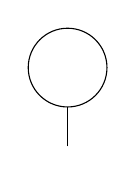
\begin{tikzpicture}[scale=0.5]
	\draw (1,0) arc[start angle=0, end angle=360, radius=1cm];
	\draw (0,-2) -- (0,-1);
\end{tikzpicture}
\end{align*}
as a subgraph is zero, since $\dim\mathcal{C}_1=0$.

Next, a loop (a circle shape) is an element in $\mathbb{C}$, called $d$.  This value must be nonzero, because the loop is the basis element of $\mathcal{C}_2$ composed with its dual.

On the other hand, the following element is in $\mathcal{C}_2$ and must thus be a scalar multiple of the single string,
\begin{align*}
\begin{tikzpicture}[scale=1, baseline]
	\node (A) at (-0.5,-0.8) {};
	\node (B) at (0.5,-0.8) {};
	\foreach \node in {A, B}
		\foreach \x in {-0.3,0,0.3} 
			\draw (\node.north) .. controls +(\x,0.5) .. ++(\x,1);
	\draw ($(A.north) + (0.3,1)$) arc[start angle=180, end angle=0, radius=2mm];
	\draw ($(A.north) + (0,1)$) arc[start angle=180, end angle=0, radius=5mm];
	\draw ($(A.north) + (-0.3,1)$) -- ++(0,0.5);
	\draw ($(B.north) + (0.3,1)$) -- ++(0,0.5);
\end{tikzpicture} \, = \, b\cdot \,
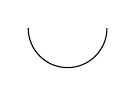
\begin{tikzpicture}[baseline]
	\draw (-0.5,0.3) arc[start angle=180, end angle=360, radius=5mm];
\end{tikzpicture}\,,
\end{align*}
and like before putting a cap on this must yield $bd\neq 0$, so the parameter $b$  must be nonzero. The trivalent vertex can be normalized so that we always take $b=1$.

Finally, we can rotate and compose trivalent vertices such that the result lives again in $\mathcal{C}_3$ (just imagine all legs bent up), and it must thus be some multiple of the trivalent vertex itself, like so:
\begin{align*}
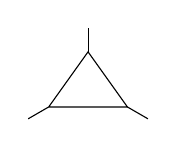
\begin{tikzpicture}[baseline]
	\coordinate (a) at (0,0.5);
	\coordinate (b) at (-0.5,-0.2);
	\coordinate (c) at (0.5,-0.2);
	\draw (a) -- ++ (0,0.3);
	\draw (b) -- ++(210:3mm);
	\draw (c) -- ++(330:3mm);
	\path[draw] (b) -- (a) -- (c) -- (b);
\end{tikzpicture}\, = t\cdot \,
\begin{tikzpicture}[baseline]
	\foreach \angle in {90, 210, 330}
		\draw (0,0) -- ++(\angle:5mm);
\end{tikzpicture}.
\end{align*}
However, coming from the composition, $t$ could actually vanish here.

\bigno In their paper, Morrison \emph{et al} then started classifying trivalent categories by
\begin{itemize}
\item[\text{a)}] the dimensions of the morphism spaces $\mathcal{C}_n$, together with
\item[\text{b)}] the parameters $d$ and $t$, often satisfying some polynomial unique to the category.
\end{itemize}

In this paper, we only look at trivalent categories where $\dim\mathcal{C}_4$ is 4-dimensional, and a basis is provided by the set of all planar trivalent graph with 4 four boundary points and no internal faces. Any trivalent category with this property is called a \emph{cubic category}.

Cubic categories have a nice relation for the square (the trivalent graph with four boundary points, four trivalent vertices, and one internal face), and that makes them particularly nice to work with.

\bigno
It is clear how to interpret open trivalent graphs with $n$-boundary points as unshaded $n$-tangles: We only need to agree on the marked points, and blow up each trivalent vertex to an internal $3$-disk, labelled with $\tau$, and we also simply call that disk $\tau$. \emph{Rotational invariance} then means $\mathrm{rot}\tau = \tau$, so the choice of marked point on $3$-disks doesn't actually matter at all.

A caveat is appropriate here: In planar algebras, we used the symbol ${}^*$ do denote the adjoint or dual of a tangle. That symbol, however, is already reserved in trivalent categories for the category-theoretic dual. Thus for a morphism $f$ in a trivalent category, $f^*$ means ``rotate through $\pi$''. Luckily, it is quickly checked that the notion of horizontally reflecting morphisms is just an instance of what has been called \emph{conjugation} before, for example in \cite{wang2010topological}, where conjugation of morphisms $f,g$ in a pivotal $\mathbb{C}$-linear category was defined as an anti-linear operation $\overline{\phantom{f}}$ that switches source and target of a morphism and satisfies
\begin{align*}
\overline{\overline{f}} = f,\qquad\qquad \overline{f\tensor g} = \overline{f}\tensor\overline{g},\qquad\qquad \overline{f\circ g} = \overline{g}\circ \overline{f}.
\end{align*}
Keeping that in mind, translating the following discussion of \emph{perfect tangles} to trivalent categories is then but a quick change in notation.